
\documentclass[11pt]{article}
    \title{\textbf{Classification of Risk Disclosures from SEC Filing Data}}
    \author{Richard Albright \\
    	Mackey RMS / InsiderScore \\
    	{\textbf{https://www.infilings.com}} \\
    	\\
    	Practicum CSE6748 \\
    	GID: 903548616}
    \date{Summer 2021}
    
    \addtolength{\topmargin}{-3cm}
    \addtolength{\textheight}{3cm}
    \usepackage{graphicx}
    \usepackage{adjustbox}
\begin{document}

\maketitle
\thispagestyle{empty}

\section{Abstract}
An implementation of a semi-supervised topic model of risk disclosures from SEC filing data.  The topics were created through the use of Latent Dirichlet Allocation and expert input.  The risk disclosures where then classified using the FastText Algorithm.  The final primary classification was determined using a cosine similarity method of classifying the risk disclosure bodies using the FastText Algorithm.  The model sampled SEC Filing Data from 2018 through the 1st quarter of 2021.  Upon creation of topics, an adjacency matrix was then created for each company's risk disclosures, then ranked according to its uniqueness across all companies within it's individual sector.  This was used to determine the particular risk disclosure's significance, and to discover filings within a company's peer group with similar risks.

\section{Introduction}
At the InsiderScore Division of Mackey RMS, we have developed a platform to speed up SEC filing data analysis \textbf{https://www.infilings.com}. The SEC mandates risk disclosures in quarterly and yearly financial statements (10-K, 10-KT, 10-Q, 10-QT), and in a company's registration statement as part of its initial public offering (S-1, S-1/A, 424B4).  A significant part of the platform is dedicated to analyzing these risk disclosure statements for a company over time, but there is currently nothing in place to compare companies' risk disclosures to their peers.  Risk disclosures are not categorized uniformly across companies, and it is up to analysts in the financial industry to make judgment calls about each risk disclosure's context and significance.  We would like to be able to categorize risk disclosures in a uniform manner based upon its context, and make an educated guess as to its significance.


\section{Problem Formulation}
The have been several attempts to classify risk disclosure statements using various natural language processing algorithms.  Most of these attempts are small in scale, and are not flexible enough to handle language that was not originally part of the models' original corpus. The model needs to be able to cope with new types of risk disclosures that it has not seen before. The company would also like to define the risk disclosure categories in a clear and concise manner, give an indication about the disclosure's significance, and eventually apply it to the full universe of filings on its platform.

\section{Approach and Implementation}
Initial potential topics were vetted using Latent Dirichlet Allocation using a random sample of 1700 risk disclosures from company 10-K and 10-Q filings from 2018 through 2020.  Initial Public Offering Filings were not used due to instability in the risk disclosure text since companies that are going public file multiple amendments during this process.  This sample set of risk disclosures and their topics was handed over to a subject matter expert to map the disclosures to the proposed categories. The subject matter expert's classifications were then used to create a class based Term Frequency - Inverse Document Frequency (TF-IDF) statistic.  TF-IDF is a statistical measure of how relevant a word is to a document in a collection of documents.  Rather than apply TF-IDF across the whole corpus, it is applied to all risk disclosures that are classified in a given class.  This will give the word embeddings that are significant to each class.  A cosine similarity matrix was created for each risk disclosure's title and body, applying the FastText word embeddings to both the category and risk disclosure's bag of words, and mapped to the category with the highest cosine similarity score.  Two supervised FastText models were also trained: one on the risk disclosure title, and one on the risk disclosure body.  The FastText models were not pretrained, and a corpus was assembled from the risk disclosures in the training set.  An ensemble model was then created out of the 3 models in an attempt to improve the accuracy further.  If 2 of the 3 models picked the same category(FastText title, FastText body, cosine similarity), that category was assigned to that particular risk disclosure. If there was no consensus for an assigned category, A ranking algorithm giving weights to the title category, the body category, and cosine similarity category was used to assign the final category to the ensemble model.    

\section{Data Pre-Processing}

The filings data was downloaded from the infilings platform using the alpha stage public API.  The data is requested via the API and returned in json format. The risk disclosure text can be in either plain text or HTML format, the API supports both modes.

\vspace{5 mm}

\begin{figure}[htp]
\centering
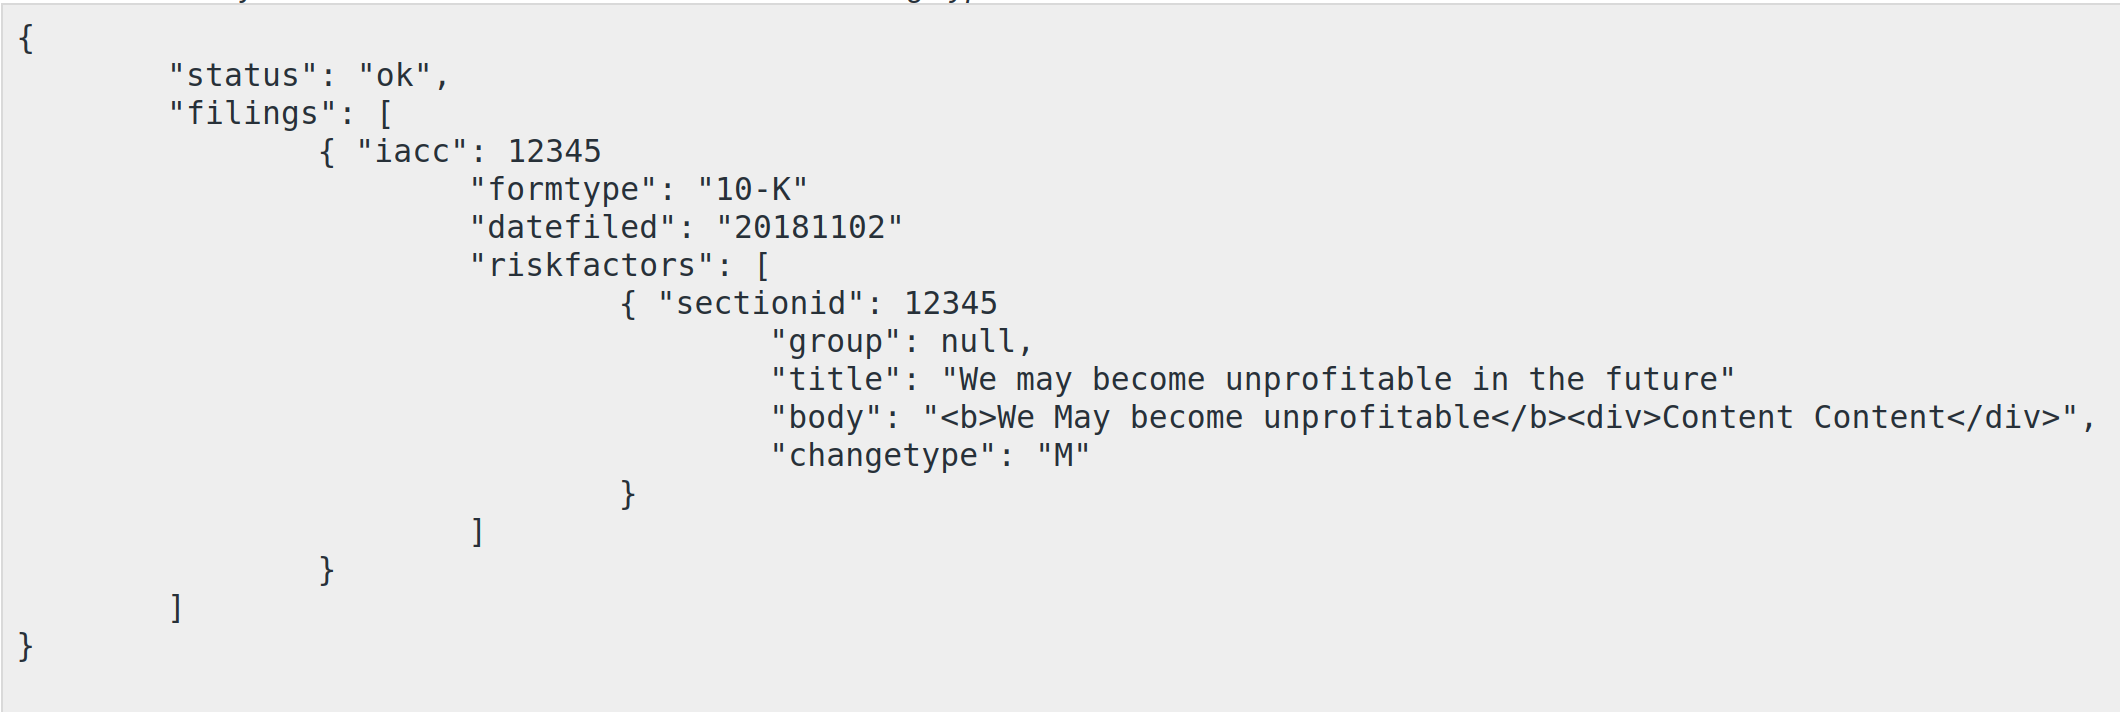
\includegraphics[scale=0.16]{images/RiskFactorContent_Json.png}
\caption{Sample of infilings JSON format}
\label{jsonformat}
\end{figure}

\vspace{5 mm}

The text was preprocessed using the spark-nlp package made available from John Snow Labs \textbf{https://johnsnowlabs.com}.  Since the performance of different levels of text preprocessing was not known beforehand, the decision was made to preprocess the entire dataset and transform each step into a spark dataframe column for testing in the proposed model.  Spark-NLP uses transformer models, even for NLP preprocessing.  The text preprocessing in spark-nlp is done via tensorflow in spark.  There are 3 fields from the JSON files that needed preprocessed: the itemtitle field, which is the risk group field in the filing, the title field, which is a summary of the risk disclosure, and the body field, which is the detailed risk disclosure.  After some initial testing, it was determined that the itemtitle and title fields could be concatenated together prior to preprocessing as there was not enough meaningful information in the itemtitle field alone.  

\vspace{5 mm}

The following preprocessing steps where then performed on the combined itemtitle + title fields (titles), and the body fields: sentence splitting, normalization, lemmatization, stemming, stop words removal, parts of speech tagging, named entity recognition tagging, and finally 2 and 3 word N-gram creation.  A gpu accelerated version of spark-nlp was used for preprocessing on a Nvidia RTX3080 10GB graphics card.  Even with gpu acceleration enabled, it was taking approximately 48 hours per year of filing risk disclosure data to preprocess the risk text. The amount of data generated by this process was enormous.  This step was taking too long and was overkill for creating a proof of concept model that would get buy in from management.  A decision was made to shorten the period of preprocessing to the years 2018 through 2021, and to limit the company's to only NYSE, AMEX, and Nasdaq listed companies.  OTC securities account for 3/4 of the filings and are not of primary concern to our clients.  This reduced the input dataset to 500MB of compressed data.  The reduction of input data resulted in the years 2018 through the 1st quarter of 2021 to be preprocessed in approximately 36 hours, and still generated approximately 125GB of preprocessed data.

\vspace{5 mm}

The initial strategy was iterate on K number of Topics using the Latent Dirichlet Allocation Method with K between 50 and 100, stepping though K every 5 topics.  Management decided that the ideal number of topics was around 80 topics, and was not interested in finding the optimal level. The topics were also going to be predetermined, and not decided by an algorithm.  In response, an 80 topic model was constructed using LDA to aide in the subject matter expert's construction of topics.  The subject matter expert then classified each risk disclosure with a main topic, and up to 3 additional acceptable topics.  The current number of topics currently sits at 90.  In order to aide in topic merging, an adjacency matrix was constructed using a cosine similarity of word embeddings to determine possible topics to be combined.  So far 6 topics have been combined down to 2, and the following topics are also under consideration for combining (topic names redacted). 

\begin{table}[h]
\centering
\begin{tabular}{ c | c | c}
  \hline
  Topic A & Topic B & Cosine Similarity \\
  \hline   
 
label 1 & label 2 & 0.6563991 \\
label 3 & label 4 & 0.59107065 \\
label 5 & label 1 & 0.5661406 \\
label 6 & label 7 & 0.5463725 \\
  \hline
\end{tabular}
\caption{Topic Word Embeddings Overlap}
\label{tbl:topic_overlap}
\end{table}

\section{Evaluation}

Three variations of a supervised FastText model have been implemented and combined into a 4th model using an ensemble method.  The model was built only using the primary tagged topic for both training and testing steps after receiving a minimal number of classified risk disclosures (1377).  There were various stages of NLP preprocessing considered as inputs into the models.  The f1-score and cross entropy loss was used for selecting the best inputs to use for the 3 models feeding the ensemble model.  The table below represents the outcome of testing various NLP preprocessing stages from worst to best f1-score.  Tokenization is prior to lemmatization, and unigrams represents lemmatization with stop words removed. Itemtitle and title columns were combined (titles) on all inputs.  Bodies were treated as a separate data point when included with the titles.

\pagebreak

\begin{table}[h]
\centering
\begin{tabular}{ c | c | c | c | c | c}
  \hline
  Preprocessing Stage & Text Input & Train Set & Test Set & F1-Score & Loss \\
  \hline    
  Unigrams & T & T & T & 0.2620 & 3.5209 \\
  Unigrams &  B & B & B & 0.3581 & 4.6289 \\   
  Lemmatization & T, B & T, B & T & 0.3886 & 0.6394 \\
  Tokenization & B & B & B & 0.5127 & 2.4484 \\                
  Tokenization & T & T & T & 0.5254 & 0.6892 \\
  Lemmatization & B & B & B & 0.5508 & 1.9684 \\
  Lemmatization & T, B & T, B & T, B & 0.5764 & 0.7231 \\
  Lemmatization & T & T & T & 0.6221 & 0.3806 \\
  Lemmatization & T, B & T, B & B & 0.7157 & 0.3226 \\


  \hline  
\end{tabular}
\caption{Evaluation of Model Inputs T=Titles, B=Body}
\label{tbl:preprocessing}
\end{table}

A supervised FastText model trained using the titles and body fields had the best f1-score when using the training set to predict the topics of the subsequent body fields in the test set.  After reaching a decision to use lemmatized text, 3 models were created.  The first model takes the titles as an input for predicting the topic of the same column. The second model used the titles and body as inputs to predict the body column. The 3rd used an adjacency matrix based on cosine similarity of the body column to model 2's trained topic word embeddings to predict the closest topic to the body text. 

\vspace{5 mm}

The models were then tested for accuracy using 5-Fold cross-validation.  The 1700 sample risk disclosures were split 80\% train (1360) and 20\% (340) test.  The training set was then split into 5 Folds.  Through the course of refining the model as new topic tags were received from the subject matter expert, the accuracy of the model using only the body text started to plateau.  That is when a decision was made to implement an ensemble method in the hopes of improving model accuracy.  It was noticed that high probability predictions on the titles text sometimes was more accurate than high probability body text.  The titles text was noticeably shorter in length than the body text, and typically contained a reference to the main topic.  It was also noticed that as more examples were added to the sample set, the similarity score of the body text to the topic word embeddings has increased substantially.  When the similarity score was first constructed with approximately 1300 samples, the accuracy was roughly 18\%, vs 76\% of the latest model.  An ensemble was then constructed to create a voting method using ranking between the titles, body, and similarity score models.  It was determined that models with a probability or similarity score of $<$ 0.70 were low quality predictions, and we do not want to display these predictions on the infiling's platform. This resulted in 19 predictions being removed from the test set, prior to creating the classification report.  Predictions were compared using the title, body, body similarity, and the new ensemble method. All classification reports left out low quality predictions in order to determine if the ensemble method performed better.

\vspace{5 mm}

An excerpt of the final results summaries from the 4 models classification report is below.


\begin{table}[h]
\centering
\begin{tabular}{ c | c | c | c | c | c}
  \hline
  Statistic & Model Type & Precision & Recall & F1-Score & Support \\
  \hline  
  accuracy & Titles & 0.6790  & 0.6790 & 0.6790 & 0.6790 \\
  macro avg & Titles & 0.6577 & 0.6378 & 0.6179 &  321 \\
  weighted avg & Titles & 0.7215 & 0.6790 & 0.6758 & 321 \\  
  accuracy & Body & 0.6481  & 0.6481 & 0.6481 & 0.6481 \\
  macro avg & Body & 0.6268 & 0.6295 & 0.6039 &  321 \\
  weighted avg & Body & 0.6570 & 0.6481 & 0.6266 & 321 \\
  accuracy & Body Similarity & 0.7601  & 0.7601 & 0.7601 & 0.7601 \\
  macro avg & Body Similarity & 0.7524 & 0.7146 & 0.7033 &  321 \\
  weighted avg & Body Similarity & 0.8344 & 0.7601 & 0.7725 & 321 \\
  accuracy & Ensemble & 0.7256  & 0.7256 & 0.7256 & 0.7256 \\
  macro avg & Ensemble & 0.6906 & 0.7209 & 0.6788 &  321 \\
  weighted avg & Ensemble & 0.7509 & 0.7256 & 0.7195 & 321 \\
  
  \hline  
\end{tabular}
\caption{Evaluation of Predicting the Topic of Body Text }
\label{tbl:classification report}
\end{table}

The model based on body similarity is the best all around in terms of precision, recall, f1-score, and accuracy.   

\vspace{5 mm}

After determining the best model above, a change in priorities from management evolved from attempting to create risk profile's of each company, to attempting to quantify the significance level of each risk disclosure in relation to its peer group.  After reaching acceptable levels of performance, the task was to then quantify the significance of a company's risk disclosure with respect to its peers.  Since comparing the risk text vs an adjacency matrix of the topic word embeddings worked fairly well, an idea to try and use cosine similarity to compare each risk disclosure with its peers on an individual basis came to surface.  Since all cosine similarities on word embeddings are positive, a whole new calculation comparing each individual risk disclosure in each sector had to be calculated per topic tag.  An accurate distance measure could not be taken by simply adding or subtracting the cosine similarity score vs the topic embeddings. A similarity matrix was then constructed for the each quarter from 2018-01-01 to 2021-03-31, broken down by sector and topic tag.  A graph was then created using the sectionid field as nodes, and the cosine similarity between 2 nodes as the weight.   A linear regression was then performed, using the graph from the 1st quarter of 2021, and the sharpe ratio's for each company for the 2nd quarter of 2021 using daily returns.  The regression compared cosine distance of each risk disclosure to its assigned topic.  If there was a consistent negative slope in relation to the cosine distance, an argument could be made for using language distance from the topic mean as a proxy for risk.  There appears to be no linear relationship between cosine distance of risk disclosures and the 3 month annualized sharpe ratio.  

\vspace{5 mm} 

\begin{figure}[htp]
\centering
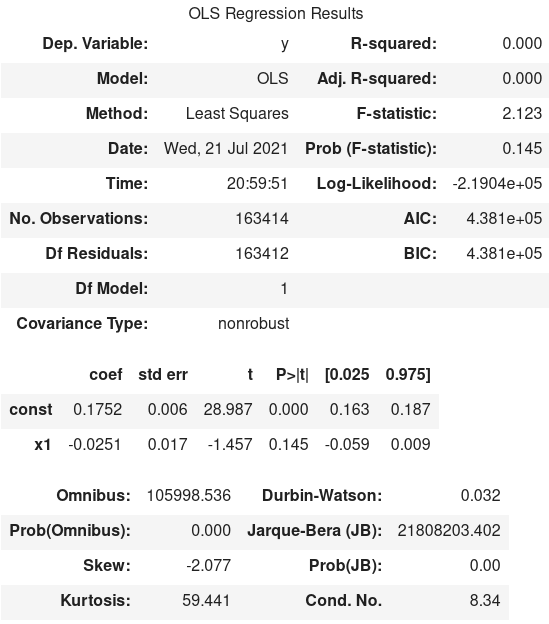
\includegraphics[scale=0.40]{images/ols.png}
\caption{Linear regression of cosine distance vs sharpe ratios}
\label{ols}
\end{figure}

\vspace{5 mm}

The graph of risk disclosure similarity is still useful and allows discovery of other company filings within the subject peer group with similar risk disclosures.  This is a desired feature for the infilings platform. This is a very basic attempt at creating a risk profile per company.  The algorithm for determining most similar filings finds all similar edges with a weight (cosine distance) of $<$ 0.20 for all risk disclosures in the source filing.  The algorithm then gets the target nodes' associated filing ids (IACC).  It returns the top 5 filings based on the top count of edges, and average weights of those edges, from the risk disclosure graph.

\vspace{5 mm}

Below is a sample of Topics Tagged on a single Risk Disclosure from Intel Corp taken from their 1st quarter 2021 10-K filing, along with the top 5 closest filings based on average distance of risk disclosures from the graph. IACCs are the internal identifier for financial filings on the infilings platform.  Results are being reviewed by data analysts by sampling individual filings for acceptable levels of performance (risk label names redacted).

\begin{table}[h]
\centering
\begin{tabular}{ c | c }
  \hline
  Key & Value\\
  \hline    
  ticker & INTC \\
  sector name & Technology \\
  industry name & Semiconductors \\
  iacc & 37227854 \\
  sectionid & 565679650 \\                
  itemtitle title words & we be subject to ip and associate with litigation... \\
  body words & we rely on access to thirdparty ip...  \\
  itemtitle title label & label 1\\
  itemtitle title prob & 0.9393\\
  body label & label 2\\
  body prob & 0.7193\\
  similarity label & label 2\\
  similarity score & 0.6216\\
  vote & label 1\\
  distance & 0.7077\\
  \hline
\end{tabular}
\caption{Sample Risk Disclosure Prediction}
\label{tbl:sample_disclosure}
\end{table}

\begin{table}[h]
\centering
\begin{adjustbox}{width=\columnwidth,center}
\begin{tabular}{ c | c | c | c | c | c }
  \hline
  iacc & ticker & sector name & industry name & risk ct & avg distance\\
  \hline
  37431823 & CRSR & Technology & Computers \& Peripherals & 18 & 0.1528 \\
  37350670 & GDDY & Technology & Internet Software \& Services & 17 & 0.1478 \\
  37382469 & PLTR & Technology & Applications \& Home Software & 17 & 0.1507 \\
  37386223 & BAND & Technology & Internet Software \& Services & 17 & 0.1636 \\
  37473766 & SMAR & Technology & Software & 16 & 0.1691 \\
  
  \hline
\end{tabular}
\end{adjustbox}
\caption{INTC Most Similar Filings Based Upon Risk Profiles}
\label{tbl:sample_disclosure}
\end{table}

\pagebreak
     
\section{Recommendations}
Management has decided to go forward with this project from the initial proof of concept, and is still interested in further developing features based on company risk profiles.  Time constraints and lack of a large training set have pushed back a more in-depth implementation of the risk profile feature.  The company currently does not have any production infrastructure for spark, and needs to be implemented to cope with the volume of data that is generated by this project.  I recommend the company implement a spark cluster in AWS' elastic mapreduce service as spot instances, with attached gpu's to speed up preprocessing.  This would include jar files for the gpu enabled spark-nlp module, as well as the jar files needed to enable the rapids spark accelerator module, which accelerates ETL on gpus.  A data lake is also suggested to be set up to hold the parquet files generated by the model, using either the hudi \textbf{https://hudi.apache.org} or delta lake \textbf{https://delta.io} projects to manage the storage layer.  The amount of data generated would be cost prohibitive to store in the database considering the access requirements by the front end, it makes much more sense to store the data in a data lake on s3 and have the data accessible from there. 

\vspace{5 mm}

 The proof of concept developed using this model was generated at quarter end, when in reality this data should be at a minimum generated nightly.  This would require tracing the risk disclosures via the threading mechanism in the database to ensure the correct risk disclosures are compared to each other at a daily point in time.  Risk disclosures from each company's 10-K annual or S-1 filings would need carried forward for risks that are not reported in the subsequent next 3 quarter's 10-Q filings in order to do an accurate comparison of risk disclosures across peer groups.  More training data is also needed, the model needs implemented as recommended above so we can embed predictions into the filing admin tool so data analysts can generate more training data as they process new filings that come in.  I look forward to further development and deployment of this model to production.


\makeatletter
\renewcommand\@biblabel[1]{\textbullet}
\makeatother

\begin{thebibliography}{shortest-entry}

\bibitem{Abrams} Abrams, Celaya-Alcalá, Baldwin, Gonda, \& Chen \textit{Analysis of Equity Markets: A Graph Theory Approach}, https://www.researchgate.net, 2016

\bibitem{Filzen} Filzen, McBrayer, \& Shannon \textit{Risk Factor Disclosures: Do Managers and Markets Speak the Same Language?}, https://papers.ssrn.com, 2016

\bibitem{Huang} Huang \textit{Exploring the Information Contents of Risk Factors in SEC Form 10-K: A Multi-Label Text Classification Application}, https://www.researchgate.net, 2010

\bibitem{Jallan} Jallan \textit{Text Mining of the Securities and Exchange Commission Financial Filings of Publicly Traded Construction Firms Using Deep Learning to Identify and Asses Risk}, https://smartech.gatech.edu, 2020

\bibitem{Lopez-Lira} Lopez-Lira \textit{Risk Factors that Matter: Textual Analysis of Risk
Disclosures for the Cross-Section of Returns}, , https://papers.ssrn.com, 2020

\bibitem{Sehrawat} Sehrawat \textit{Learning Word Embeddings from 10-K Filings
for Financial NLP Tasks}, https://papers.ssrn.com, 2019

\bibitem{Walkowiak} Walkowiak \& Gniewkowski \textit{Evaluation of vector embedding models in clustering of text documents}, https://www.researchgate.net, 2019

\bibitem{Zhang} Zhang, Gao, Fang, \& Zhang \textit{Enhancing Short Topic Modeling with FastText Embeddings}, https://ieeexplore.ieee.org 2020

\bibitem{Zolotov} Zolotov \& Kung \textit{Analysis and Optimization of fastText Linear Text Classifier}, https://arxiv.org, 2017

\end{thebibliography}
\end{document}

